\documentclass[14pt,A4]{article}
    % \usepackage{minted}
    % \usepackage{amsmath}
    \usepackage{amsthm}
    \usepackage{amsfonts}
    \usepackage[margin=0.5in]{geometry}
    \usepackage{enumitem}
    \usepackage{graphicx}
    \usepackage{float}


    \title{Project 3 \\
        \large CSE 574}
    \author{Alec Friedman and Zesheng Wang}
    
    \begin{document}
    \maketitle
    \section*{One-vs-all Logistic Regression}
    For this project we implemented logistic regression to classify handwritten digits. Since logistic regression typically deals with binary classification, in order to classify digits in classes from 0-9 we had to implement the one-vs-all strategy. This means we assign an element $x$ to the class with the maximum posterior probability. After training, we observed a 92.75\% classification accuracy on training data, 91.49\% accuracy on validation data, and 92.02\% accuracy on test data.

    \section*{Multi-class Logistic Regression}
    We also implemented multi-class logistic regression as an additional part of the project. The results for multi-class logistic regression were 93.098\% accuracy on training data, 92.42\% accuracy on validation data, and 92.53\% accuracy on test data. These results were slightly more accurate than the one-vs-all strategy. Additionally, training was significantly faster than for the one-vs-all strategy. This is due to the fact that the one-vs-all strategy requires multiple iterations of training to take place, each iteration classifying yes or no for each individual class. This leads to $k$ training iterations, where $k$ is the number of classification classes, as opposed to one training step for multi-class logistic regression

    \section*{Support Vector Machine}
    For the final portion of this project, we utilized the sklearn.svm module to create a support vector machine. We ran this svm with various parameters and kernel functions. When running with linear kernel, training takes significantly shorter than with the radial basis function kernel. When the gamma value was set to 1 with the rbf kernel, results were incredibly poor. However, with the default gamma value, the rbf kernel outperformed the linear kernel in terms of accuracy. Linear kernel yielded a 93.78\% accuracy on the test data, while rbf kernel with default parameters yielded 94.42\% accuracy. When increasing C values for the svm, we can see that accuracy dramatically increases from 1 to 20. However after that point, while it does continue to increeas in accuracy, this increase becomes much less significant in size for the validation and test data. The training data continues to increase in accuracy, although this is less important than the validation and test data.

    \begin{figure}[H]
        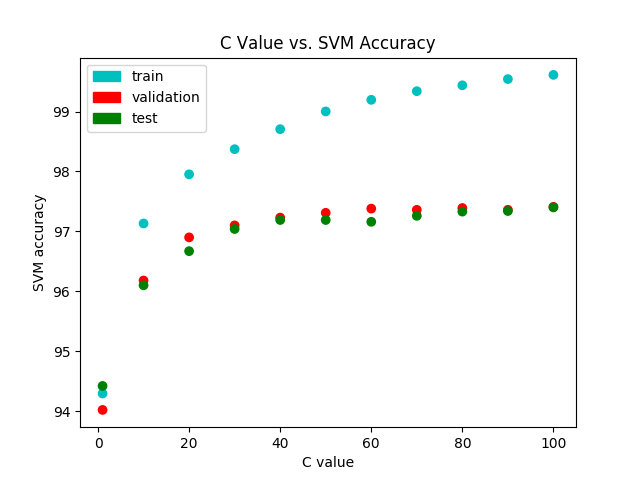
\includegraphics[width=\linewidth]{./results/results.png}
        \caption{Support Vector Machine accuracy varying C values}
        \label{fig:plots3}
    \end{figure}

    \end{document}